\documentclass[12pt]{article}
\usepackage{fullpage,enumitem,amsmath,amssymb,graphicx,url,hyperref}
\usepackage{sectsty}

\hypersetup{
    colorlinks=true,
    linkcolor=blue,
}

\sectionfont{\fontsize{15}{20}\selectfont}

\DeclareMathOperator*{\argmax}{arg\,max}
\DeclareMathOperator*{\argmin}{arg\,min}
\DeclareMathOperator{\E}{\mathbb{E}}
\usepackage{tgpagella}

\begin{document}

\begin{center}
{\Large \textbf{CS330 Autumn 2023 Homework 1 \\ Data Processing and Black-Box Meta-Learning}}
\\ {\large Due Wednesday October 16, 11:59 PM PST}

\begin{tabular}{rl}
SUNet ID: &  \\
Name: & \\
Collaborators: & 
\end{tabular}
\end{center}

By turning in this assignment, I agree by the Stanford honor code and declare
that all of this is my own work.

\section*{Overview}

\textbf{Goals:} In this assignment, we will look at meta-learning for few shot classification. You will:
\begin{enumerate}
    \item Learn how to process and partition data for meta learning problems, where training is done over a distribution of training tasks $p(\mathcal{T})$.
    \item Implement and train memory augmented neural networks, a black-box meta-learner that uses a recurrent neural network \cite{pmlr-v48-santoro16}.
    \item Analyze the learning performance for different size problems.
    \item Experiment with model parameters and explore how they improve performance.
\end{enumerate}

We have provided you with the starter code, which can be downloaded from the course website. We will be working with Omniglot~\cite{Lake1332}, a dataset with 1623 characters from 50 different languages. Each character has 20 28x28 images.
We are interested in training models for $K$-shot, $N$-way classification, i.e. training a classifier to distinguish between $N$ previously unseen characters, given only $K$ labeled examples of each character.

\vspace{0.2cm}
\noindent\textbf{PDF Submission}: To submit your homework, submit one PDF report to Gradescope containing written answers and Tensorboard graphs (screenshots are fine) to the questions below. The PDF should also include your name and any students you talked to or collaborated with. \textbf{Any written responses or plots to the questions below must appear in your PDF submission.} 

\vspace{0.2cm}
\noindent\textbf{Code Submission.}
You should only modify the following two files:
\begin{itemize}
    \item \texttt{submission/load\_data.py}
    \item \texttt{submission/mann.py}
\end{itemize}
However, when submitting to Gradescope, you should \textbf{include all the files} inside your \texttt{submission} folder, which includes those \texttt{.npy} files. \textbf{Please only submit the files but not the \texttt{submission} folder.}

\vspace{0.2cm}
\noindent\textbf{Optional. Autograding Your Code.}
In this homework, we include autograding functionalities in the released code to facilitate you to debug and develop your code. To run the autograder, simply do:

\texttt{python grader.py}

\noindent The maximum points you can get when running the autograder is \textbf{15 / 15 points}. We also have \textbf{27 points} from hidden test cases that show up when you submit your code to Gradescope. This makes the total of \textbf{42 points} for all the Coding parts. Note that some of the test cases require you to have the \texttt{mann\_results\_*.npy} files ready, which are auto-generated when you finished all the four runs required by \textbf{Problem 3}.



\section*{[15 points (Coding)]\\Problem 1: Data Processing for Few-Shot Classification}

Before training any models, you must write code to sample batches for training. Fill in the \texttt{\_sample} function in the \texttt{DataGenerator} class in \texttt{load\_data.py}. The class already has variables defined for batch size \texttt{batch\_size} ($B$), number of classes \texttt{num\_classes} ($N$), and number of samples per class \texttt{num\_samples\_per\_class} ($K+1$). Your code should:
\begin{enumerate}
    \item Sample $N$ different characters from either the specified train, test, or validation folder.
    \item Load $K+1$ images per character and collect the associated labels, using $K$ images per class for the support set and 1 image per class for the query set.
    \item Format the data and return two tensors, one of flattened images with shape [$K+1, N, 784$] and one of one-hot labels [$K+1, N, N$].
\end{enumerate}  

\begin{figure}
    \centering
    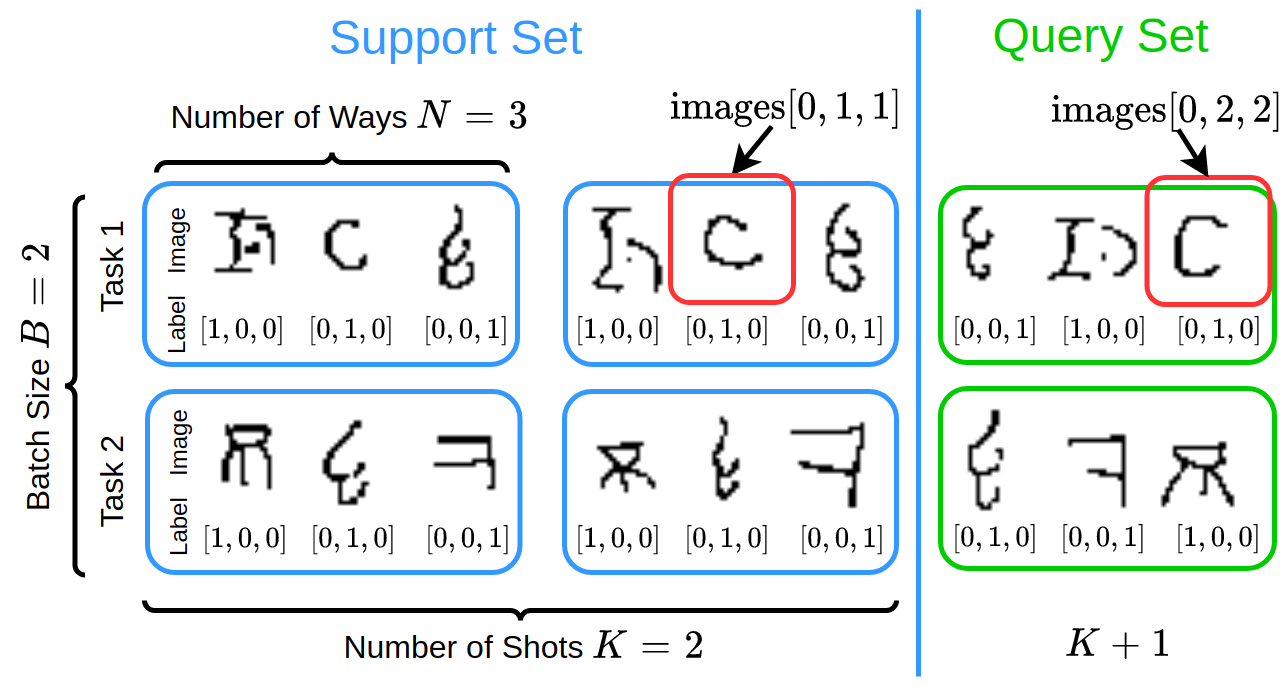
\includegraphics[width = 0.75\textwidth]{figures/hw1_batch_v4.png}
    \vspace{-0.3cm}
    \caption{\small Example data batch from the Data Generator. The first $K$ sets of images form the support set and are passed in the \emph{same order}. The final set of images forms the query set and must be shuffled.}
    \label{fig:batch}
\end{figure}
Note that your code only needs to return one single (image, label) tuple. 

You \textbf{do not need to handle batching in function} since we can basically batch the inputs using an instance of torch.utils.data.DataLoader for multiple tasks, and the final shape input images to your MANN model is thus [$B, K+1, N, 784$], and that of the input labels is [$B, K+1, N, N$], where B is the batch size. Check the declaration of \texttt{meta\_train\_iterable} and \texttt{meta\_train\_iterable} in \texttt{main.py} on how we use your implemented \texttt{DataGenerator}. 

Figure \ref{fig:batch} illustrates the data organization. In this example, we have: (1) images from $N=3$ different classes; (2) we are provided $K=2$ sets of labeled images in the support set and (3) our batch consists of only two tasks, i.e. $B=2$. 
\begin{enumerate}
    \item We will sample both the support and query sets as a single batch, hence one batch element should obtain image and label tensors of shapes $[K+1, N, 784]$  and $[K+1, N, N]$ respectively. In the example of Fig. \ref{fig:batch}, \texttt{images[0, 1, 1]} would be the image of the letter "C" in the support set with corresponding class label $[0, 1, 0]$ and \texttt{images[0, 2, 2]} would be the the letter "C" in the query set (with the same label).

    \item We must shuffle the order of examples in the \textbf{query set}. In principle, you should be able to shuffle the order of data in the support set as well; however, this makes the model optimization much harder. \textbf{You should feed the support set examples in the same, fixed order}. In the example above, the support set examples are always in the same order. Note here that images and labels should be shuffled
    in the same order, otherwise, the one-to-one mapping between images
    and labels may get messed up. Hint: we encourage you to use np.random.shuffle here.

\end{enumerate}

\noindent We provide helper functions to (1) take a list of folders and provide paths to image files/labels, and (2) to take an image file path and return a flattened numpy matrix. The functions \texttt{np.random.shuffle} and \texttt{np.eye} will also be helpful. \textbf{Be careful about output shapes and data types!}




\section*{[15 points (Coding)]\\Problem 2: Memory Augmented Neural Networks (MANN)     \cite{pmlr-v48-santoro16,DBLP:journals/corr/MishraRCA17}}

We will now be implementing few-shot classification using memory augmented neural networks (MANNs). The main idea of MANN is that the network should learn how to encode the first $K$ examples of each class into memory such that it can be used to accurately classify the $K+1$th example. See Figure~\ref{mann} for a graphical representation of this process.

Data processing will be done as in SNAIL~\cite{DBLP:journals/corr/MishraRCA17}. Each set of labels and images are concatenated together, and the $N*K$ support set examples are sequentially passed through the network as shown in Fig. \ref{mann}. Then the query example of each class is fed through the network, \textbf{concatenated with 0 instead of the true label}. The loss is computed between the query set predictions and the ground truth labels, which is then backpropagated through the network. \textbf{Note}: The loss is \textit{only} computed on the set of $N$ query images, which comprise of the last examples from each character class. 

\begin{figure}
\centering
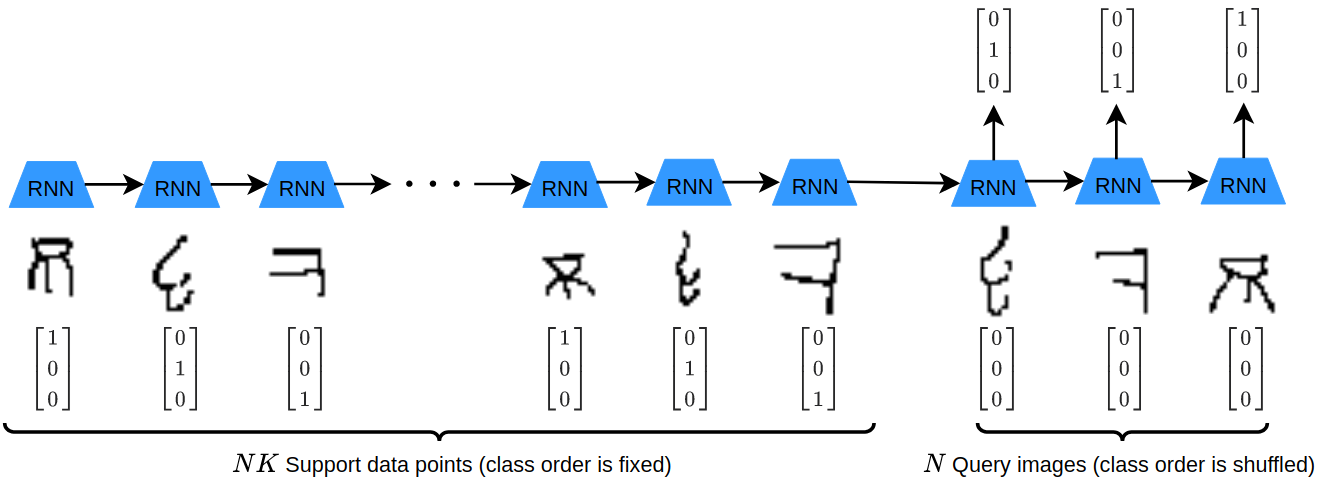
\includegraphics[width=\linewidth]{figures/hw1seq.png}
\vspace{-9mm}
\caption{Feed $K$ labeled examples of each of $N$ classes through the memory-augmented network. Then feed final set of $N$ examples and optimize to minimize loss.}
\label{mann}
\end{figure}



\noindent In the \texttt{mann.py} file:
\begin{enumerate}
    \item Fill in the \texttt{forward} function of the \texttt{MANN} class to take in image tensor of shape [$B, K+1, N, 784$] and a label tensor of shape [$B, K+1, N, N$] and output label predictions of shape [$B,K+1,N, N$]. The layers to use have already been defined for you in the \texttt{\_\_init\_\_} function, and you can just call them in your \texttt{forward} code. \textit{Hint: Remember to pass zeros, not the ground truth labels for the final $N$ examples.}
    \item  Fill in the function called \texttt{loss\_function} in the \texttt{MANN} class which takes as input the [$B,K+1,N, N$] labels and [$B,K+1,N, N$] predicted labels and computes \href{https://pytorch.org/docs/stable/generated/torch.nn.functional.cross_entropy.html#torch.nn.functional.cross_entropy}{the cross entropy loss} only on the $N$ test images. 
\end{enumerate}
\textbf{Note}: Both of the above functions will need to be backpropogated through, so they need to be written in PyTorch in a differentiable way.


\section*{[12 points (Coding)][4 points (Plot)][6 points (Written)]\\Problem 3: Analysis}

Once you have completed problems 1 and 2, you can train your few shot classification model. You should observe both the support and query losses go down, and the query accuracy go up. Now we will examine how the performance varies for different size problems.
Train models for the following values of $K$ and $N$:
\begin{itemize}
    \item $K = 1$, $N=2$ %, you should be able to achieve about 90\% accuracy.
    \item $K = 2$, $N=2$ %, you should be able to achieve about 80\% accuracy.
    \item $K = 1$, $N=3$ %, you should be able to achieve about 75-80\% accuracy.
    \item $K = 1$, $N=4$ %, you should be able to achieve about 70\% accuracy.
\end{itemize}

Example code:

\textcolor{green}{\texttt{python main.py --num\_shot K --num\_classes N}}

For checking training results and/or taking a screenshot for the writeup, use:

\textcolor{green}{\texttt{tensorboard --logdir runs/}}

You should start with the case $K=1 , N=2$ as it can aid you in the implementation and debugging process. Your model should be able to achieve a query set accuracy of above 90\% in this first two scenarios scenario on held-out test tasks, around 80\% in the second scenario, and more than 60\% in the final scenario.

\textbf{Note: The computation of this homework should be doable on your laptop's CPU. For reference, running one experiment takes around $3mins$ on our TA's Apple MacPro M1.} 



Answer the following questions:

\begin{enumerate}
    \item \textbf{[4 points (Plot)]} For each configuration, submit a plot of the meta-test query set classification accuracy over training iterations (A \href{https://pytorch.org/docs/stable/tensorboard.html}{TensorBoard} screenshot with all plots in Figure is fine).
    
    \textcolor{red}{Your plot goes here.}

    \item \textbf{[2 points (Written)]} In our problem, we shuffled the order of examples in the query set. Do we really need to perform this step? What happens if we do not shuffle?

    \textcolor{red}{Your answer goes here.}
    
    \item \textbf{[2 points (Written)]} How does increasing the number of classes affect learning and performance?
    
    \textcolor{red}{Your answer goes here.}
    
    \item \textbf{[2 points (Written)]} How does increasing the number of examples in the support set affect performance?
    
   \textcolor{red}{Your answer goes here.}
    
\end{enumerate}

\section*{\textbf{[5 points (Plot, Written)][5 points (Extra Credits)]}\\
Problem 4: Experimentation}
\begin{enumerate}[label=\alph*]
    \item \textbf{[5 points (Plot, Written)]} Experiment with one hyperparameter that affects the performance of the model, such as the type of recurrent layer, size of hidden state, learning rate, or number of layers.  Submit a plot that shows how the meta-test query set classification accuracy of the model changes on 1-shot, 3-way classification as you change the parameter. Provide a brief rationale for why you chose the parameter and what you observed in the caption for the plot. \textbf{If you aim to do the following Extra Credit question, you need to test something different than the LSTM hidden dimension here.}

    
    \textcolor{red}{Your plot and answer goes here.}
    
    
    \item \textbf{[5 points (Extra Credit)]} In this question we'll explore the effect of memory representation on model performance. We will focus on the $K=1$, $N=3$ case.
    
    In the previous experiments we used an LSTM model with 128 units. Consider additional memory sizes of 256, and 8. How does increasing and decreasing the memory capacity influence performance?
    
    \textcolor{red}{Your plot and answer goes here.}
    
\end{enumerate}

\newpage
\bibliography{references}
\bibliographystyle{unsrt}

\end{document}
